\documentclass[tikz,border=5pt]{standalone}
\pdfinfoomitdate=1
\pdftrailerid{}
\pdfsuppressptexinfo=-1
\usepackage{pgfplots}
\usepgfplotslibrary{groupplots}
\pgfplotsset{compat=1.18}
\pgfplotsset{colormap/viridis}
\definecolor{atlas0}{HTML}{0072B2}
\definecolor{atlas1}{HTML}{D55E00}
\definecolor{atlas2}{HTML}{009E73}
\definecolor{atlas3}{HTML}{E69F00}
\definecolor{atlas4}{HTML}{56B4E9}
\definecolor{atlas5}{HTML}{CC79A7}
\definecolor{atlas6}{HTML}{000000}
\definecolor{atlas7}{HTML}{F0E442}
% NATO SERS figure F41; data_sha256=9c8bd012684fd017f5ff1e96f2d5ab5822148827a84341b7a731485ee370688d
% caption=(S) RQ-P01 C09 confusion structure. Cells are row-normalized within each technical repeat after pooling eligible held domains, then averaged across five repeats; frozen tables retain the repeat minimum and maximum. Spectrum support is observations; master support is domain-master membership after instrument-balanced aggregation. Colour uses a perceptually uniform scale. This diagnostic does not treat spectra or repeats as independent evidence.
\begin{document}
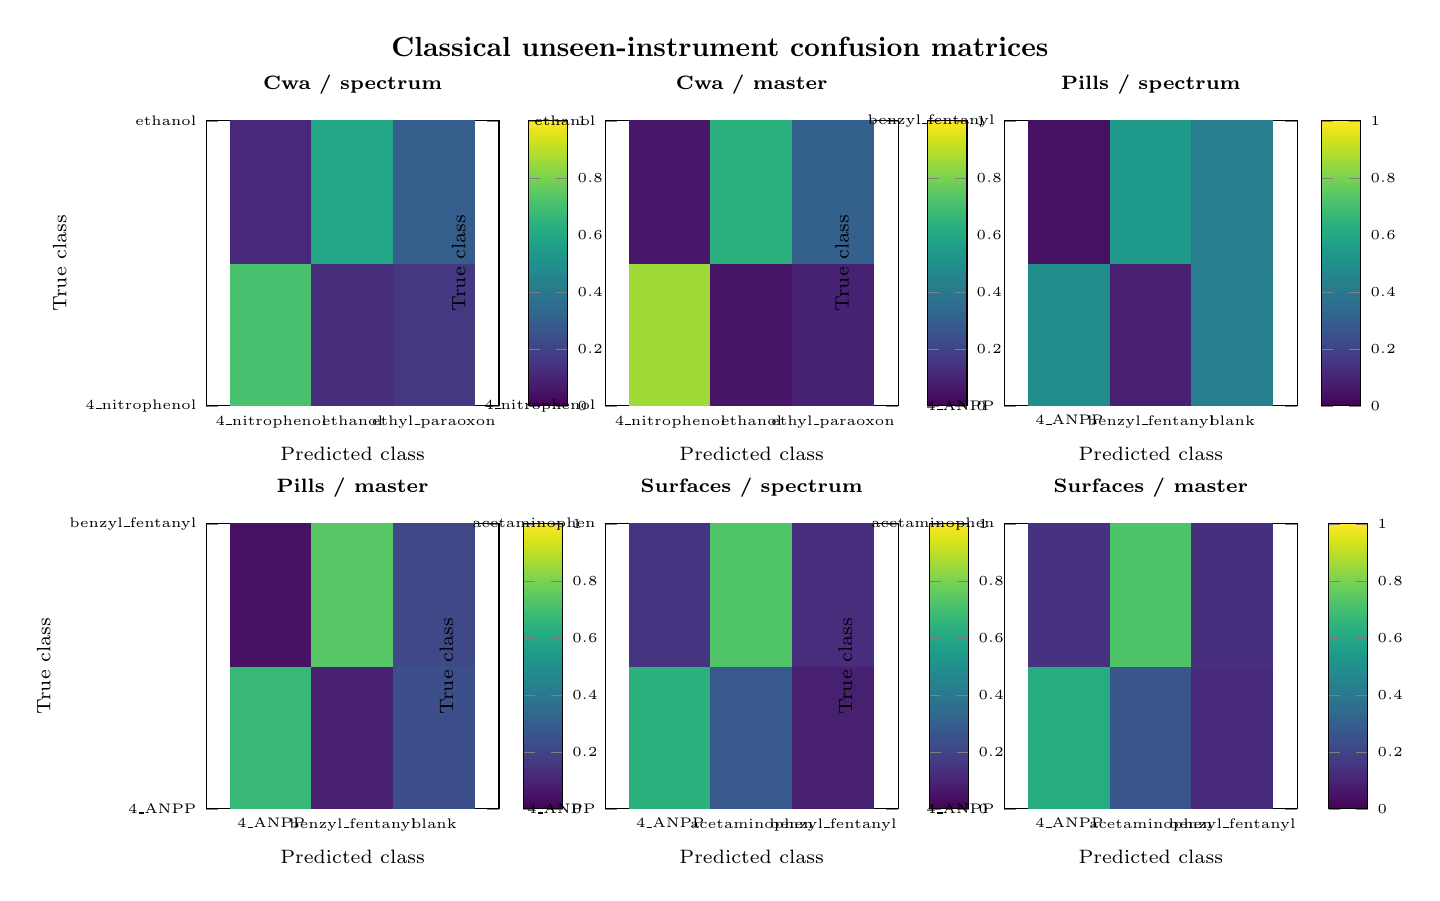
\begin{tikzpicture}
\begin{groupplot}[group style={group size=3 by 2, horizontal sep=1.35cm, vertical sep=1.5cm}, width=5.30cm, height=5.2cm, grid=major, tick label style={font=\tiny}, label style={font=\scriptsize}, title style={font=\scriptsize\bfseries,align=center}, legend style={font=\tiny,draw=none,fill=white,fill opacity=0.9,text opacity=1}]
\nextgroupplot[title={Cwa / spectrum},xlabel={Predicted class},ylabel={True class},ymin=0,ymax=1,xtick={0,1,2},xticklabels={4\_nitrophenol,ethanol,ethyl\_paraoxon},ytick={0,1,2},yticklabels={4\_nitrophenol,ethanol,ethyl\_paraoxon},point meta min=0,point meta max=1,colorbar]
\addplot[matrix plot*,mesh/cols=3,point meta=explicit] coordinates {(0,0) [0.711224] (1,0) [0.12854378] (2,0) [0.16023222] (0,1) [0.11151842] (1,1) [0.59362084] (2,1) [0.29486074] (0,2) [0.24045541] (1,2) [0.3716888] (2,2) [0.38785579]};
\nextgroupplot[title={Cwa / master},xlabel={Predicted class},ylabel={True class},ymin=0,ymax=1,xtick={0,1,2},xticklabels={4\_nitrophenol,ethanol,ethyl\_paraoxon},ytick={0,1,2},yticklabels={4\_nitrophenol,ethanol,ethyl\_paraoxon},point meta min=0,point meta max=1,colorbar]
\addplot[matrix plot*,mesh/cols=3,point meta=explicit] coordinates {(0,0) [0.85833333] (1,0) [0.05] (2,0) [0.091666667] (0,1) [0.058333333] (1,1) [0.63777778] (2,1) [0.30388889] (0,2) [0.21976912] (1,2) [0.32611833] (2,2) [0.45411255]};
\nextgroupplot[title={Pills / spectrum},xlabel={Predicted class},ylabel={True class},ymin=0,ymax=1,xtick={0,1,2},xticklabels={4\_ANPP,benzyl\_fentanyl,blank},ytick={0,1,2},yticklabels={4\_ANPP,benzyl\_fentanyl,blank},point meta min=0,point meta max=1,colorbar]
\addplot[matrix plot*,mesh/cols=3,point meta=explicit] coordinates {(0,0) [0.48888889] (1,0) [0.086111111] (2,0) [0.425] (0,1) [0.041666667] (1,1) [0.5375] (2,1) [0.42083333] (0,2) [0.017073171] (1,2) [0.053658537] (2,2) [0.92926829]};
\nextgroupplot[title={Pills / master},xlabel={Predicted class},ylabel={True class},ymin=0,ymax=1,xtick={0,1,2},xticklabels={4\_ANPP,benzyl\_fentanyl,blank},ytick={0,1,2},yticklabels={4\_ANPP,benzyl\_fentanyl,blank},point meta min=0,point meta max=1,colorbar]
\addplot[matrix plot*,mesh/cols=3,point meta=explicit] coordinates {(0,0) [0.67058824] (1,0) [0.088235294] (2,0) [0.24117647] (0,1) [0.043478261] (1,1) [0.73913043] (2,1) [0.2173913] (0,2) [0] (1,2) [0.045] (2,2) [0.955]};
\nextgroupplot[title={Surfaces / spectrum},xlabel={Predicted class},ylabel={True class},ymin=0,ymax=1,xtick={0,1,2},xticklabels={4\_ANPP,acetaminophen,benzyl\_fentanyl},ytick={0,1,2},yticklabels={4\_ANPP,acetaminophen,benzyl\_fentanyl},point meta min=0,point meta max=1,colorbar]
\addplot[matrix plot*,mesh/cols=3,point meta=explicit] coordinates {(0,0) [0.6367894] (1,0) [0.2781145] (2,0) [0.085096094] (0,1) [0.14882228] (1,1) [0.72606917] (2,1) [0.12510855] (0,2) [0.13105904] (1,2) [0.31048003] (2,2) [0.55846093]};
\nextgroupplot[title={Surfaces / master},xlabel={Predicted class},ylabel={True class},ymin=0,ymax=1,xtick={0,1,2},xticklabels={4\_ANPP,acetaminophen,benzyl\_fentanyl},ytick={0,1,2},yticklabels={4\_ANPP,acetaminophen,benzyl\_fentanyl},point meta min=0,point meta max=1,colorbar]
\addplot[matrix plot*,mesh/cols=3,point meta=explicit] coordinates {(0,0) [0.61583593] (1,0) [0.26320268] (2,0) [0.12096139] (0,1) [0.14213156] (1,1) [0.72319566] (2,1) [0.13467278] (0,2) [0.097870546] (1,2) [0.24032982] (2,2) [0.66179963]};
\end{groupplot}
\node[font=\normalsize\bfseries,anchor=south] at (current bounding box.north) {Classical unseen-instrument confusion matrices};
\end{tikzpicture}
\end{document}
